\documentclass[../main.tex]{subfiles}
\graphicspath{{\subfix{../images/}}}
\begin{document}

Our nutrition is composed of multiple basic building blocks, which each in turn have very different
tasks to perform in our body.

the beginning and end of a healthy nutrition is to combine the basic building blocks in a sensible way and it helps us
to maintain our body to the be lean, healthy and full of power into a high age.

These basic building blocks of our food are:
\begin{itemize}
\item Water
\item Proteins
\item Fats (lipids)
\item Carbohydrates (sugar, starch)
\item Vital substances
\item Fibers
\end{itemize}

\begin{table}[htb!]
  \centering
  \begin{tabular}{lcccc}
    \textbf{Building Block} & \textbf{kJ/g} & \textbf{kcal/g} & \textbf{kJ/oz} & \textbf{kcal/oz} \\
    Proteins & 17 & 4 & 482 & 113 \\
    Fats & 37 & 9 & 1049 & 255 \\
    Carbohydrates & 17 & 4 & 482 & 113 \\
  \end{tabular}
  \caption{Energy content of the different building blocks of our food}
\end{table}

\section{Water}

\begin{figure}[htb!]
  \centering

\includegraphics[width=5cm]{GlassWater.eps}
  \caption{A glass of water~\cite{GlassWater}}
\end{figure}



Water doesn't contain any nutrients, but nevertheless is water of the biggest importance for the human body.
Without water, there's no life.
The human body consists our of about 60\% water (a newborn even up to 75\%).
Roughly 60\% of that water is found in the intracellular space (inside the cells).
The rest is in between the cells in the form of interstitial fluids (between the cells),
like blood plasma, lymph, urine, saliva, digestion fluids, tear liquid, nose secretes and sweat.


In the human organism, water mainly serves:
\begin{itemize}
\item to cover the needs of fluids in cells and tissues,
\item as a solvent and medium of transportation for nutrients, enzymes, hormones and so on,
\item to excrete metabolism end products over the urine,
\item to regulate the body temperature.
\end{itemize}

\subsection{How much Water does a Human Being Need?}

During a day, the human body looses\index{water consumption} 2--2.5 liters (8\sfrac{1}{2}\ -- 10\sfrac{1}{2}\ cups) of water, of which:
\begin{itemize}
\item 1.0 -- 1.5 L (4\sfrac{1}{4}\ -- 6\sfrac{1}{4}\ cups) through the urine
\item 0.4 -- 1.0 L (1\sfrac{3}{4}\ -- 4\sfrac{1}{4}\ cups) through respiration
\item 0.1 -- 0.5 L (3\sfrac{1}{2}\ fl.oz. -- 2\sfrac{1}{8}\ cups) over the skin, through sweat
  \item 0.1 -- 0.2 L (3\sfrac{1}{2}\ -- 7 fl.oz.) through feces
  \end{itemize}

  This loss of water has to be added back to our body on a daily base, through drinking and eating.
  For a healthy, barely physical active person, that means a daily fluid intake of about 30 -- 35 mL of fluids per kg (0.45 -- 0.54 fl.oz./lbs) body weight.
  A person who weights 70 kg (154 lbs) therefore needs a fluid supply of 2.0 -- 2.5 L (8\sfrac{1}{2}\ -- 10\sfrac{1}{2} cups) per day.
  Out of this amount, about 0.5 -- 1 L (2\sfrac{1}{8}\ -- 4\sfrac{1}{4} cups) fluids will be supplied through food (veggies, fruits, \ldots).
  This results then in the recommended amount of drinking about 1 -- 2 L (one to two quarts) of fluids a day.

  Please consider, that the water usage also depends on the outside temperature, physical activity levels and the state of health.
  When it's hot, under heavy physical labor or sport, sweating will cool down the body and
  in case of disease (fever, diarrhea, vomiting) the body will also loose a lot of additional water.
  All these losses need to be compensated with additional fluid intake.

  \subsection{Is Water the Best Drink?}

  As drinks counts foods, which pretty much only furnish water to our body. 
  Fruit and veggie juices, milk, yogurt drinks and soft drinks deliver next to water plenty of nutrients and energy and  don't really count as drinks.
  Alcoholic drinks are non--essential food items, stimulants and are very bad at hydrating our body.
  On top of that, they are delivering a lot of unwanted energy (about 7 kcal/g, roughly 200 kcal per oz.).

% Swiss tap water - US tap water?
  
  Pure water is by far the best and cheapest drink. Tap water, depending on location filtered, is the best option to hydrate.
  In order to change things up, can water be flavored in different ways:
  \begin{itemize}
  \item Fruit or herbal tea
  \item Black or green tea* 
  \item Broth
  \item Coffee*
    \item Lemon water (juice of one lemon for one Liter (quart) of water)
  \end{itemize}
{\footnotesize{*See special drinks and foods in the section \ref{SpecialFoods}, page~\pageref{SpecialFoods}.}}
  
People who are depended on bottled water, should preferably choose still water.
  The carbonation leeches vital oxygen from our body and adds unnecessary acids to our system.

  \subsection[Drinking Too Little, Too Much or the Wrong Drinks]{People Who Drink Not Enough, Too Much or the Wrong Things Risk their Health}

  Humans can survive multiple weeks without food, but without fluids only three days.
  Already a loss of fluids of 1\% or our body weight leads to the first symptoms like head ache, difficulties focusing and thirst.
  Being thirsty already indicates a lack in fluids.
  With advances age, the thirst signal decreases, which in turn is the reason that older people often don't drink enough.
  Among other effects, this leads to:
  \begin{itemize}
  \item higher viscosity of the blood, with the danger of thrombosis and a decreased oxygen supply of the organs
  \item dry skin, which is easier to be hurt
  \item drier mucous membranes, which are more susceptible to infections
    \item constipation, through excessive thickening of the feces
    \end{itemize}

    An excessive intake in fluids also can threaten the physical productivity and in excess even get dangerous.
    But the biggest danger comes from the many calories, if soft drinks or alcoholic drinks get consumed in excess. 

 
\vspace{5mm}
\noindent
\begin{fminipage}{\textwidth}
  \textbf{Profile Water}
  \begin{itemize}
  \item The human body consists of 60 \% of water and a human can only survive three days without water intake
  \item Water is vital for humans, it transports nutrients, enzymes and hormones to the cells; it helps the excretion of harmful substances and the regulation of the body temperature
  \item Water is free of calories and doesn't deliver energy to the body
  \item We need about 2 -- 2.5 L (8\sfrac{1}{2}\ -- 10\sfrac{1}{2}\ cups) of fluids a day, thereof 1 -- 2 L (1 -- 2 quarts) in the form of water
    \item Preferably pure water or mineral water without carbonation
  \end{itemize}
\end{fminipage}

\section{Proteins}

\begin{figure}[htb!]
\centering
  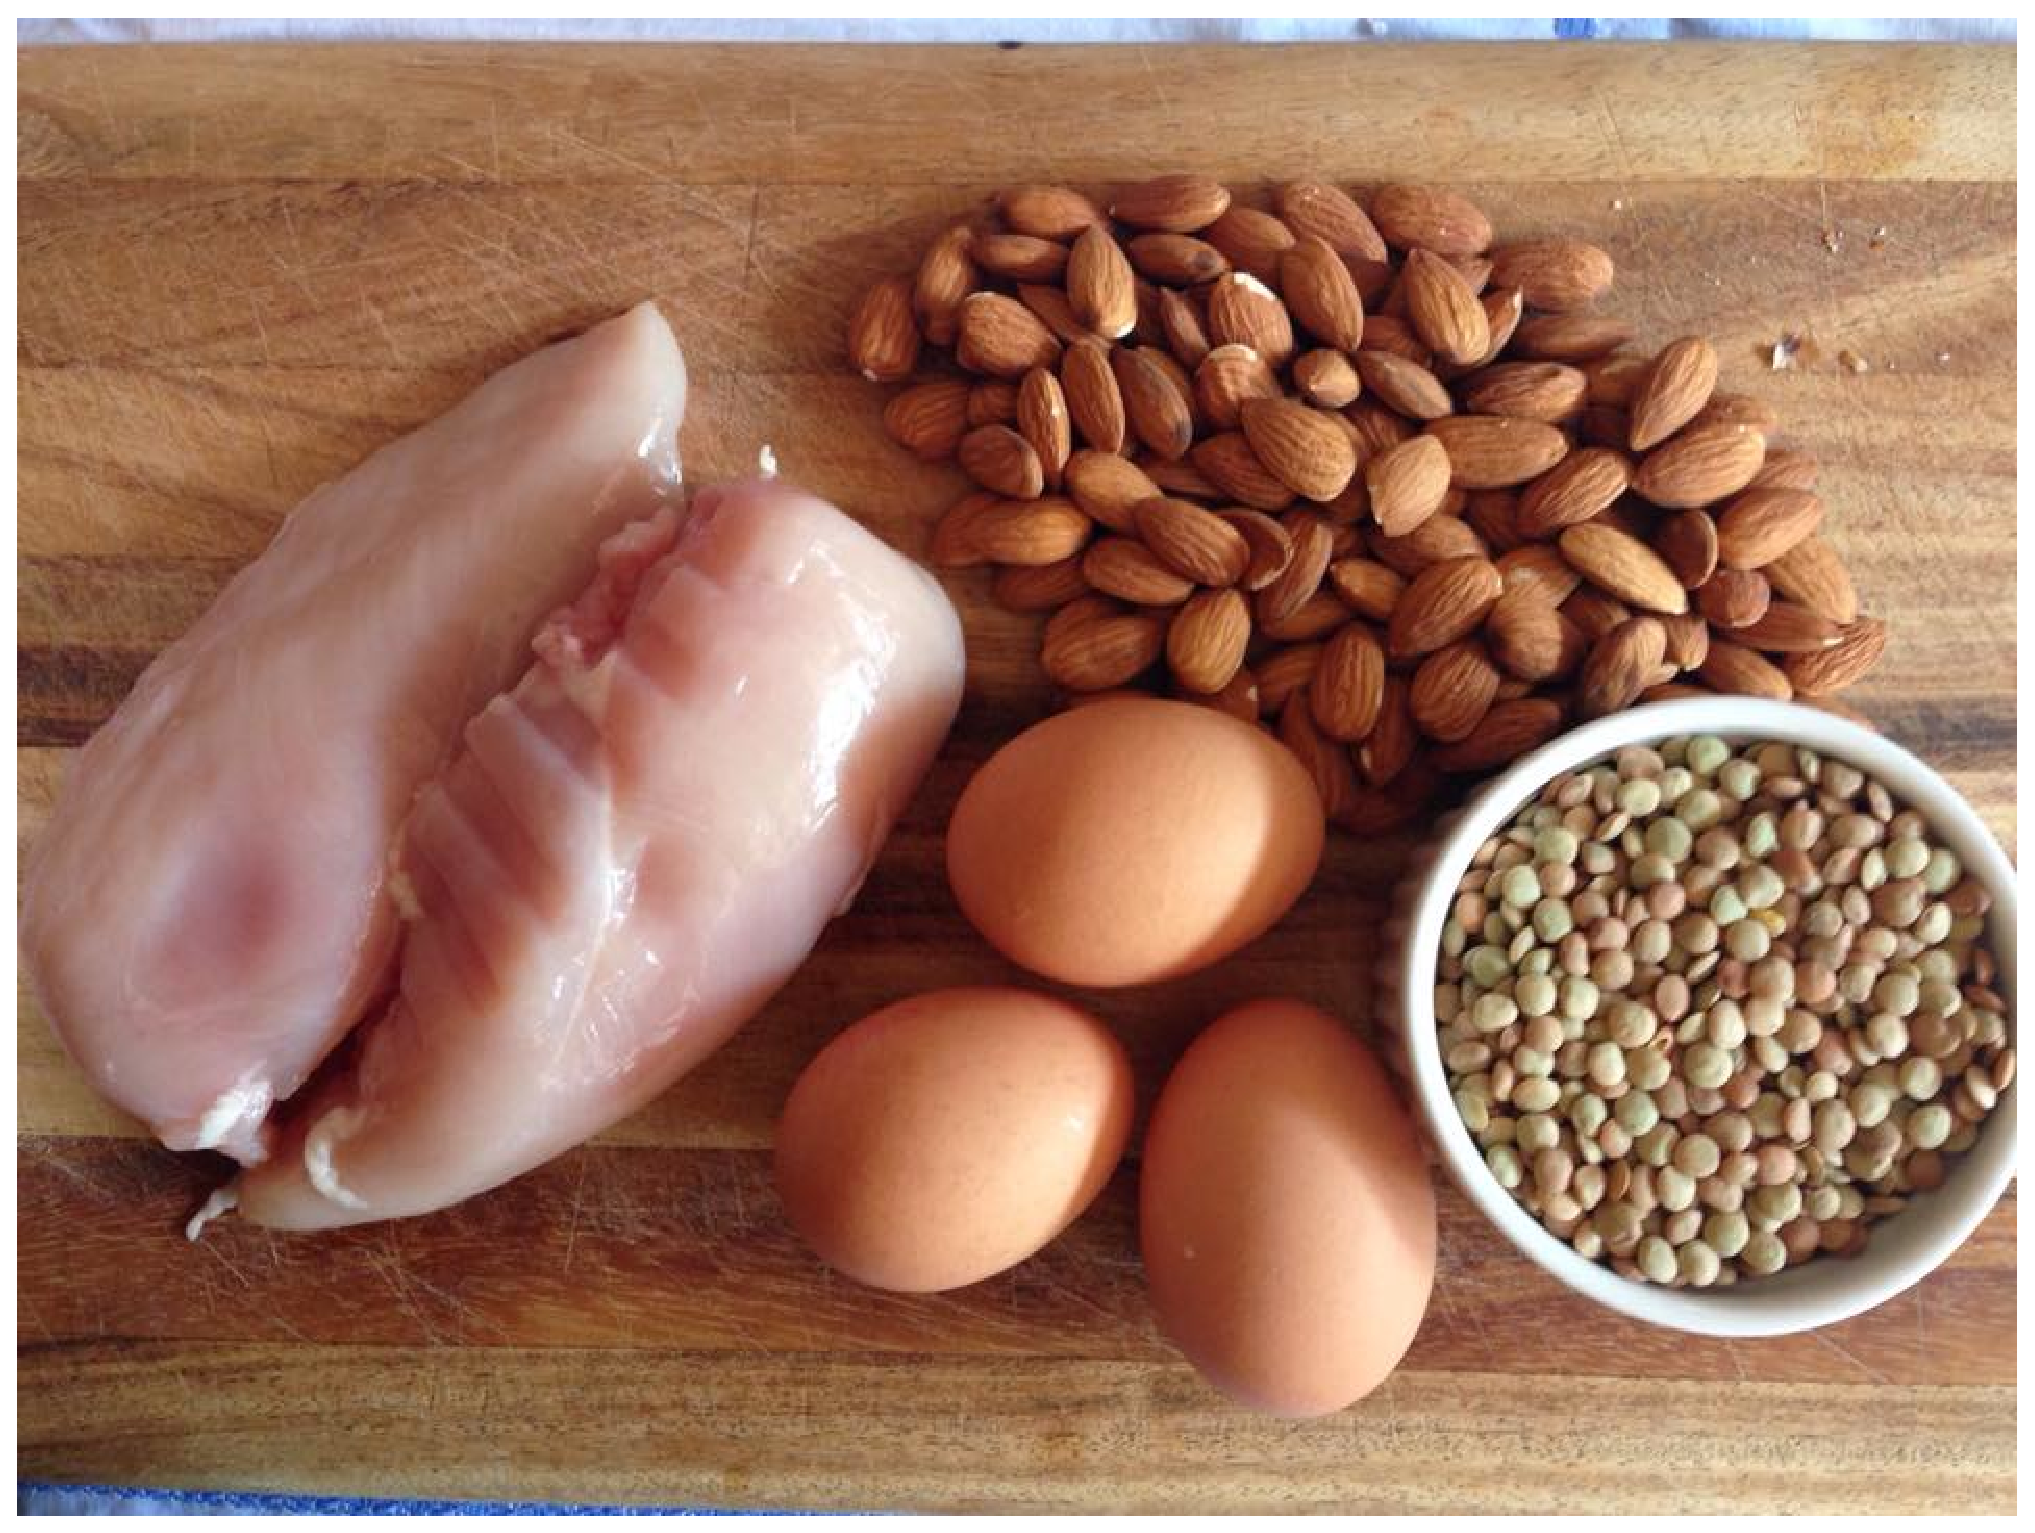
\includegraphics[width=7cm]{Protein-rich_Foods}
  \caption{Protein rich foods\cite{Proteins}}
  % It says from wikipedia https://upload.wikimedia.org/wikipedia/commons/e/e8/Protein-rich_Foods.jpg
\end{figure}

First and foremost, are proteins building blocks to build up our bodies.
Proteins are the basic building blocks of every single one of our cells, of muscles, connective tissue, skin,
blood, internal organs, hormones and enzymes.
Given that the body cells get constantly renewed and built up again and again, we humans require a constant supply of proteins.
A lack in proteins can lead to a dismantlement of important parts of the body.
But too much proteins isn't good either.
Excessive proteins can only be stored in our bodies to a very limited amount.
So superfluous proteins, or their degradation products urea and uric acid, have to be excreted over the kidneys.
This in turn can overburden the kidneys and lead to rheumatism and gout.
Only secondarily are proteins used for energy.
As carbohydrates, they deliver 4 kcal or 17 kJ of energy per gram (113 kcal or 482 kJ per oz.).

Proteins have very different roles in our body. A selection:
\begin{itemize}
\item in the form of collagen (about \sfrac{1}{3} of the body's proteins), they build up the structure of the skin, connective tissue and the bones
\item in our muscles, myosin and actin change their shapes and by doing doing lead to contractions of the muscles and allow us to move
\item enzymes organize and execute the bio--catalytic functions, that means they allow  and control specific (bio)chemical reactions in our body
\item as transport proteins, they organize the transport of vital substances like for instance hemoglobin, which organizes the transport of oxygen in the blood stream
\item as antibodies, they serve to combat infections
  \item as reserves, they serve the body as energy supply in the case of hunger.
  \end{itemize}

  \subsection{The Structure of Proteins}

  Proteins\index{protein} are nitrogen containing organic substances, which consist out of different long chains of coupled amino acids\index{amino acids}.
  There are 20--22 different amino acids knows, which the human organism needs.
  Thereof, 8 amino acids and in special situations 9--10 (for instance children, sick people) are essential for the human organism.
  That means that we can't build them up ourselves and need to take them in with our food in the form of proteins.

  \begin{table}[htb!]
    \centering
    \begin{tabular}{l|l}
      \multicolumn{2}{c}{\textbf{Amino acids}} \\
      \textbf{not essential} & \textbf{essential} \\
      \hline
      Alanine & Isoleucine \\
      Arginine** & Leucine \\
      Asparagine & Lysine \\
      Aspartic Acid & Methionine \\
      Cysteine & Phenylalanine \\
      Glutamine & Threonine \\
      Glutamic Acid & Tryptophan \\
      Glycine & Valine \\
      Histidine**\\
      Proline\\
      Serine\\
      Tyrosine*\\
      \hline
      \multicolumn{2}{l}{\footnotesize{*essential for infants and pregnant women}}\\
      \multicolumn{2}{l}{\footnotesize{**essential for adolescents and sick people}}
    \end{tabular}
    \caption{The individual amino acids}
  \end{table}

  \subsection{The Eight Essential Amino Acids}

  Almost all fruits and veggies contain most of those eight essential amino acids.\index{amino acids!essential}
  But there are fruits and veggies which contain all of those amino acids, which the human body can't produce.
  Those foods are: carrots, banana, cauliflower, cabbage, Brussels sprouts, corn, cucumber, egg plants, peas, potatoes, sweet potatoes and tomatoes.
  Additionally, all nuts, sun flower and sesame seeds, peanuts and beans contain all 8 essential amino acids.
  The content of usable amino acids is way higher in plants than in meats as foods.
  At the end of the chapter, you find a table with foods which contain a lot of proteins.\footnote{These weights are
    quite small and almost impossible to translate to ounces (oz). Maybe grains or drachms might make sense, but in my experience they aren't used that often
    and people in the USA are unfamiliar with their use. When using this table, please convert your own calculations, with 1 oz = 28.35 g.}
  

  \begin{table}[htb!]
    \centering
    \begin{tabular}{lllll}
      \multicolumn{5}{l}{\textbf{Protein intake (daily)}} \\
      \multicolumn{5}{l}{Guide value in g per kg body weight (reference values DACH 2000)}\\
      \hline
      Children & Girls & 0.9 g & Boys & 0.9 g \\
      Adolescents & Girls & 0.8 g & Boys & 0.9 g \\
      Adults & Women & 0.8 g & Men & 0.8 g \\
      Pregnant & after 4th month & 10 g/day & additional \\
      Breast feeding &  & 10 g/day & additional \\ 
    \end{tabular}
    \caption{How much proteins do human beings need?}
  \end{table}

  \subsection{Protein Deficiency}

  In the industrialized nations, a deficiency of proteins is very rare and only occurs in diets which are very protein poor.
  The average western mixed diet contains about 100 g (3\sfrac{1}{2}\ oz.) of proteins, which is more than sufficient.

  The effects of a lack of an insufficiency in proteins are:\index{protein!deficiency}
  \begin{itemize}
  \item Loss of hair (Hair consists of 97 -- 100 \% of proteins --- Keratin)
  \item Degradation of muscles and muscle weakness
  \item Immune-- insufficiency and infections
  \item In the worst case, it can lead to the protein--deficiency disease Kwashiorkor\index{symptom!Kwashiorkor}.
    People (mostly children) suffering from Kwashiorkor can be recognized through their so called hunger--belly,
    which is caused by an excessive storage of water (edemas).
    \item Ongoing lack of proteins leads to death.
  \end{itemize}

  \subsection{Proteins are the First Choice ``Weight Loss Helpers''}

  Karl Lagerfield pretty much cut himself in two with proteins: he lost 42 kg (92\sfrac{1}{2} lbs) in one year!\index{protein!weight loss}
  Also science knows, if diets do work, then the protein diets, our of the following reasons:
  \begin{itemize}
  \item Proteins holds the muscles back from destroying themselves. And the person undergoing the diet will need the muscles  to burn the fat.
  \item Proteins lead to a feeling of saturation
    \item Proteins lead to burning fat
    \end{itemize}

    \subsection{Proteins are a Fat Burner}

    If you drink a glass butter milk and have a lean piece of poultry or fish, your body has to add energy to transform these food proteins into body proteins.\index{weight loss}
    Where is your body getting this energy from? From the fat reserves.
    One gram of food proteins has 4 kcal and 25\%, therefor 1 kcal has to be added by your body in order to use the protein.
    Your body depletes the fat depots for the required energy.
    In order to use this fat burner effect and that it truly shows on the balance you have to be mindful that you prefer healthy and lean sources of protein.

    \subsection{``Good'' and ``Bad'' Proteins}

    At this point you might ask yourself: When this substance is that valuable, why does it then have such a bad reputation?
    Mostly, because our sources of protein consist mostly of red meat (pork and beef), sausage and creamy sauces.
    They don't only provide amino acids, but also cholesterol, fats and purine (poison).

    Better, healthy, sources of proteins are eggs, fish, white meat (poultry, veal, rabbit), venison, legumes, soy, nuts, grains and milk products.
    Plant based proteins aren't as valuable for our body like animal proteins, due to the patterns of amino acids.
    But the quality can be easily improved, by combining the right foods. For instance adding an egg to a vegetarian meal greatly enhances the
    biological availability of the amino acids.

    \subsection{Deficit of Protein Despite of the Abundance}

    Many people suffer from a deficit of proteins, even though they eat a lot of proteins, because they nourish themselves the wrong way.
    Given that vital substances are missing, they can't produce enough stomach acid or enzymes to cleave the proteins into amino acids.
    That way, the valuable amino acids don't arrive at their intended destination: the cells.
    When the proteins don't get cleaved into the small bits, it can't be admitted to the blood.
    Undigested proteins remain in the colon, leads to difficulties with digestion and
    allergic reactions.\index{symptoms!allergy}\index{symptom!digestion troubles}
    The lack of proteins makes fat and sick.
    That won't happen to you anymore as you know now, to be mindful about what you put into your system.

    \subsection{Heads Up: Trap!}

    Now you might think: proteins make you loose weight.
    Well, so I'm going to eat only proteins and no carbohydrates --- and I'm going to loose a lot of weight. 
    It works, many different crash diets are based on that principle.
    These diets recommend proteins and forbid carbohydrates --- and sure enough you are loosing a lot of weight.
    But, it's only water that you're loosing.
    Your metabolism doesn't go along with that, it switches to a hunger program, called ``ketose''.\index{ketose}
    Triggered by a high supply of proteins an lacking carbohydrates, your body produces so called ketones.
    These ketones are being excreted over the kidneys along with a lot of water.
    That's not bad in itself and is part of your biological programming.
    But the dieting success on the balance shows that's it's mostly water that you loose, not fat.

    You can do it better --- combine!

    Eat proteins with carbohydrates: fish with wild rice or veggies, tofu with pasta, cheese with a piece of whole grain bread,
    cream cheese with fruits.
    By doing so, you are refueling enough sugar for the brain.
    Your body is neither forced to activate the metabolic pathway of ketosis nor to digest the muscles.
    That way, your body depletes fat depots to change the valuable protein to invest
    into youthfulness, immune system, muscles, power und into happiness.
    \begin{itemize}
    \item Combine grains (rice, buckwheat, wheat, oats, spelt, barley, rye, sorghum) with legumes (beans, soy, garbanzo beans/chickpeas, peas, lentils).
      That's the reason, why in Mexico a staple is rice and beans. In Europe: cream cheese with potatoes.
    \item Another way to improve the quality of the protein: grains with egg, milk or milk products (Yogurt, cream cheese, cheese).
      \item Yet another clever way to combine: potatoes with egg, milk or milk products.
      \end{itemize}

      \subsection{Happiness = Proteins and Carbohydrates}

      Important: if dieting, then with  happiness.
      There's another reason why you should combine proteins with carbohydrates.
      Carbohydrates by themselves make you tired, they inhibit the activity of the brain.
      In the brain, chemical messengers, so called neurotransmitters are being build in response, which tend to induce tiredness.
      Proteins avoid that proteins make you tired.
      Proteins deliver the amino acid tyrosine and produces from that invigorating chemical messengers of the good feelings:
      dopamine and norepinephrine.\index{dopamine}\index{norepinephrine}
      These substances make happy, you are able to think faster, you are more alert, motivated and mentally active --- and in a way better mood.
\end{document}